\documentclass[11pt,a4paper]{article}

\usepackage[utf8]{inputenc}
\usepackage[english]{babel}
\usepackage[T1]{fontenc}

\usepackage{amsmath,amssymb,amsfonts}

\usepackage{hyperref}
\usepackage{graphicx}

\title{Computational Geometry - Exercises for week 1}
\author{Philip Munksgaard\\Sebastian Paaske Tørholm}

\begin{document}
\maketitle

\section{Exercise 1.3}
Let $E$ be the set of edges, and $\mathcal{P}$ be the (initially empty) list of
ordered points in the polygon.

First, create $P$, a sorted array of the endpoints of the edges, each tagged
with the edge they belong to. This takes $O(n \lg n)$.

Pick an edge $e_0$, to be our starting edge, and let $e_0 = (p_0, p_0')$.

Do a binary search on $P$ for $p_0$, finding the other edge ending in $p_0$. Let
$p_1$ be the other endpoint of this edge.

Check if $p_0', p_0$ and $p_1$ together make a right turn. If so, add $p_0'$ and
$p_0$ to $\mathcal{P}$. Let $p_{start} = p_0'$.

If they do not make a right turn, locate the edge corresponding to $p_0'$ in
$P$, and let $p_1'$ be the other edgepoint, in a similar fashion as to what
was done for $p_1$. $p_0$, $p_0'$ and $p_1'$ must now make a right turn, so add
$p_0$ and $p_0'$ to $\mathcal{P}$. Let $p_{start} = p_0$.

For $i$ starting at $1$, ending when $p_i \neq p_{start}$, repeat the following: 
\begin{itemize}
    \item Add $p_i$ to $\mathcal{P}$
    \item Find the other edge containing $p_i$ using binary search on $P$. Let $p_{i+1}$
          be the other endpoint of this line.
\end{itemize}

After this, $\mathcal{P}$ contains the clockwise polygon corresponding to the
edges in $E$.

\section{Exercise 1.6}

\subsection{a}
Let $L$ be a set of line segments and $E$ be the set of endpoints of the lines in $L$.

We wish to prove that $CH(L) = CH(E)$.

Since $E \subseteq L$, and $L \subseteq CH(L)$, we must have $E \subseteq CH(L)$. Since
$CH(E)$ is the smallest such convex set, we must have that $CH(E) \subseteq CH(L)$.

We now need that $CH(L) \subseteq CH(E)$. By definition of convexity, we know that for any
$p_1$ and $p_2$ in $E$ the line $p_1p_2 \subseteq CH(E)$. Since each line in $L$ has this
form, we must have that $L \subseteq CH(E)$. By same argument as above, we get $CH(L) \subseteq CH(E)$.

This proves that $CH(L) = CH(E)$.

\subsection{b}

As seen in \autoref{counterexample}, we cannot simply use the method used by
Graham's scan directly to solve the problem.

\begin{figure}[h!]
    \centering
    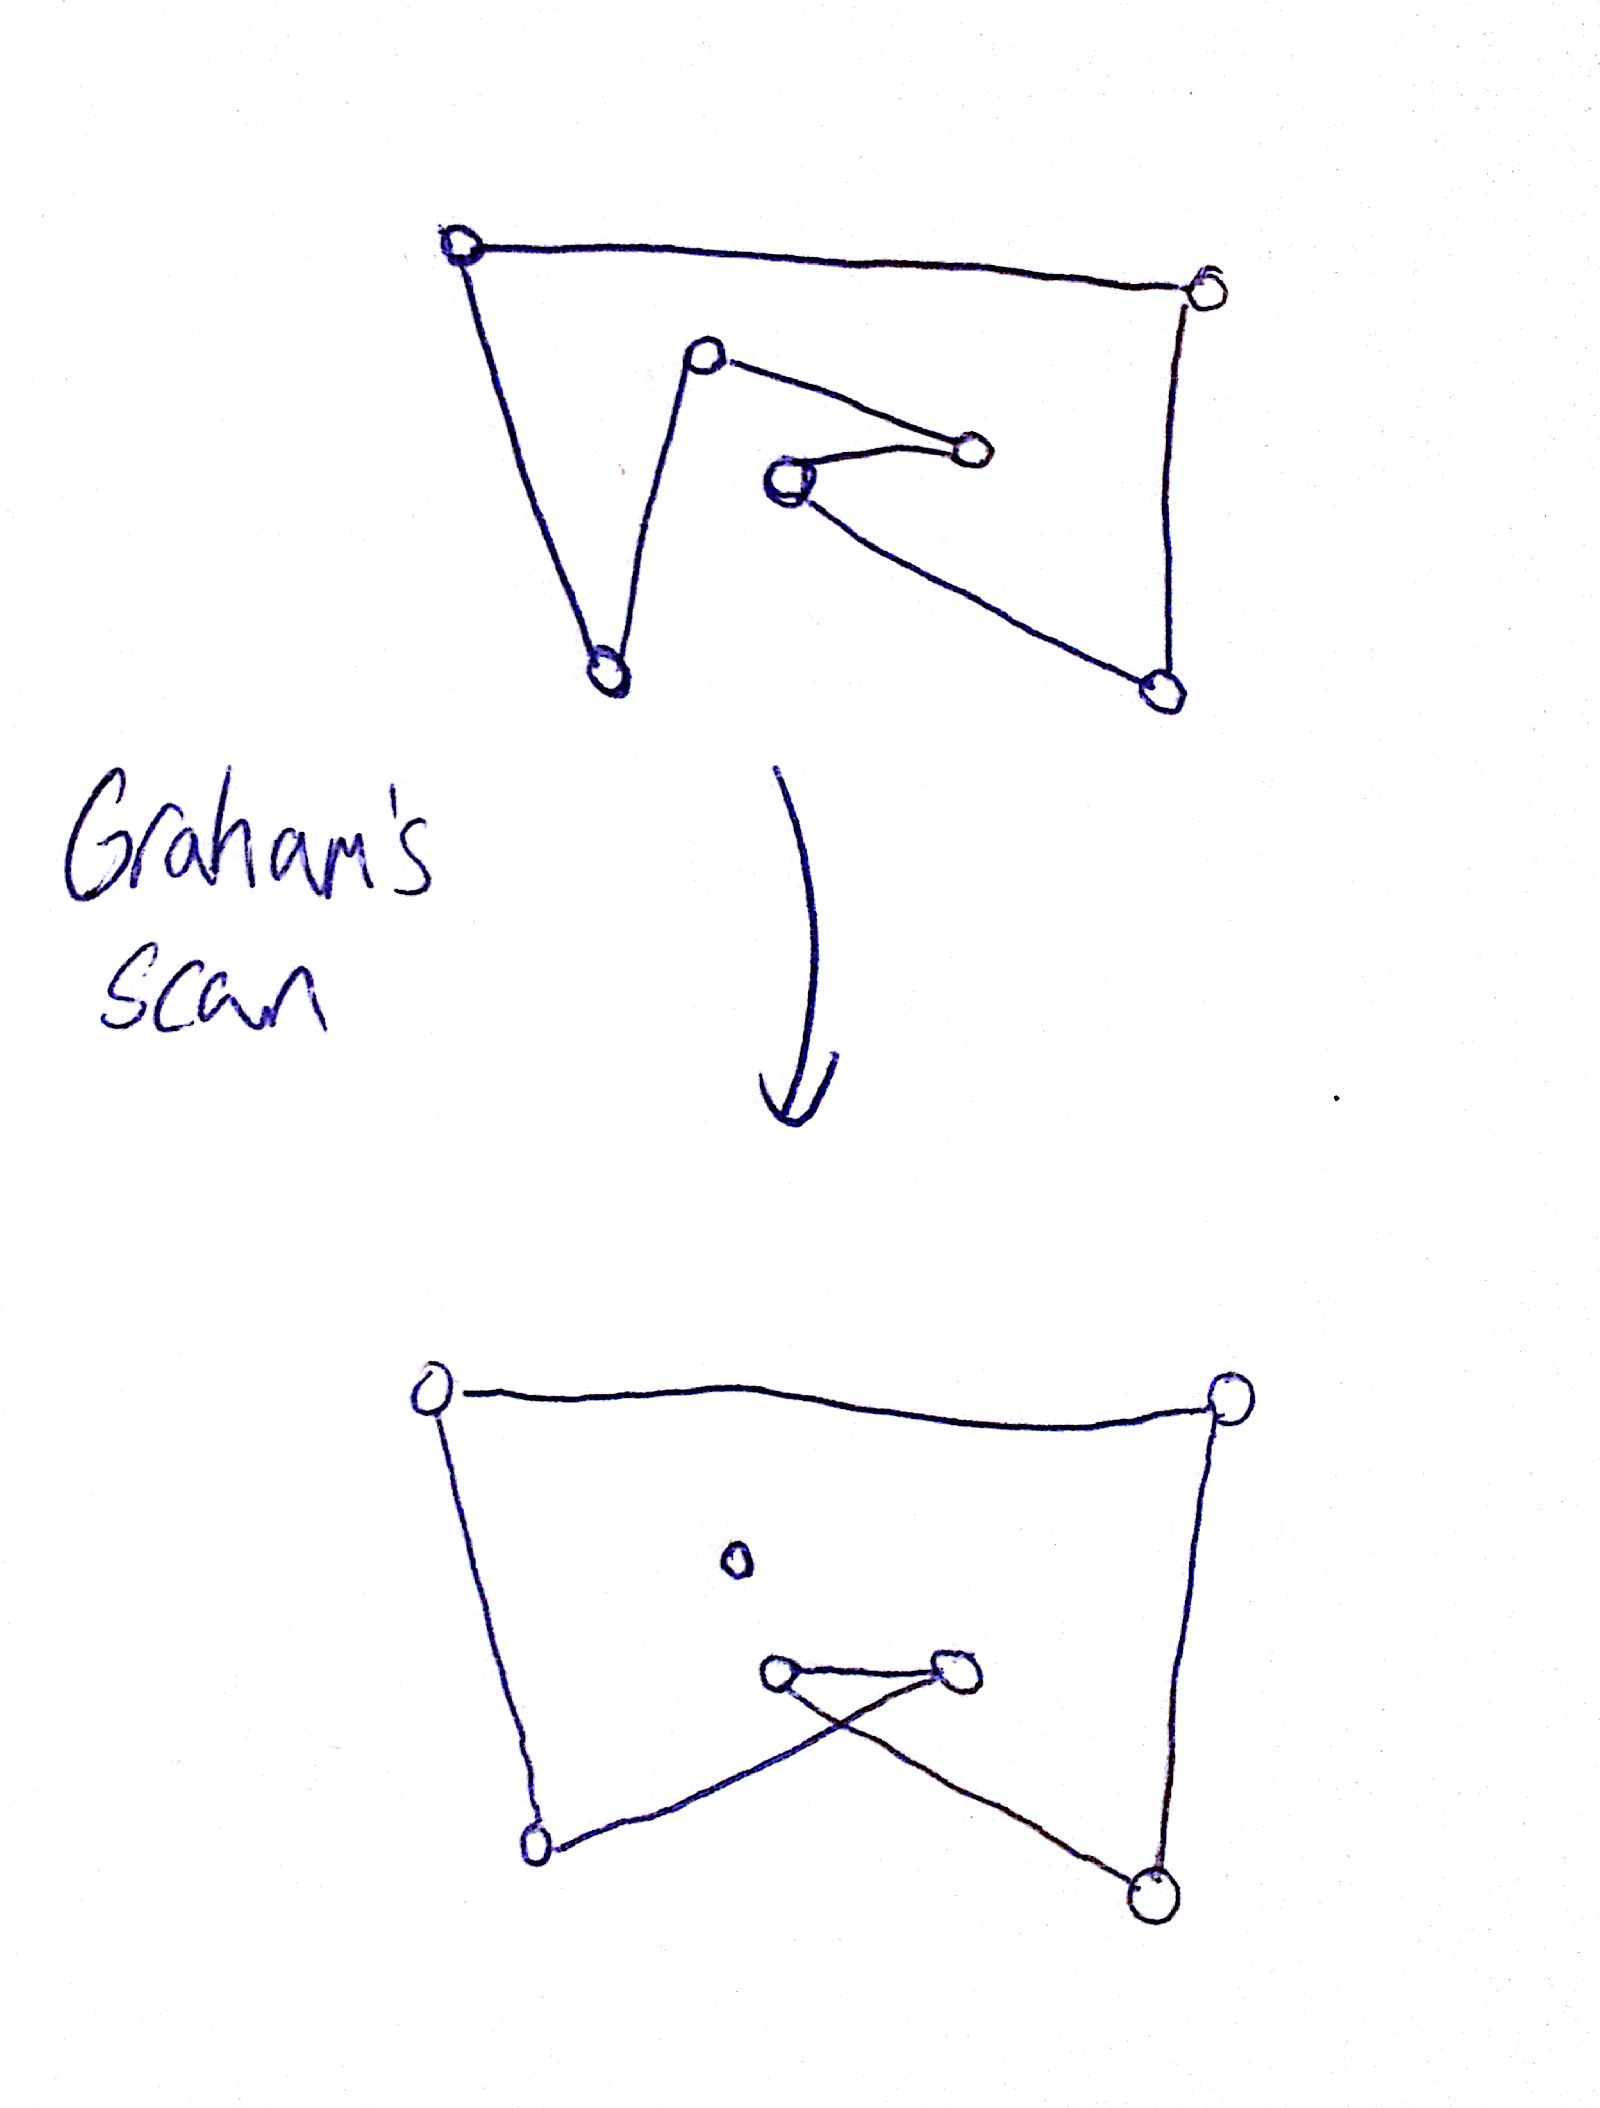
\includegraphics[width=.5\textwidth]{counterexample.jpg}
\caption{Counter example showing that Graham's scan directly does not solve the problem.}
\label{counterexample}
\end{figure}

We observe that violating the constraint that the points need to be given in sorted order
introduces problems, allowing it to degenerate a simple polygon to a non-simple one.

Instead we base our approach on the algorithm ConvexHull from the book. 

First we determine the leftmost and rightmost point. These two points partition the polygon into two parts, one of which we will convert to the bottom hull, and one of which we will convert to the top hull. Determining which is which\footnote{Equivalent to determining if polygon is clockwise or counter clockwise in relation to the two extreme points.} is simple. Simply take one extreme point and look one point in each direction. Since we know the polygon doesn't self-intersect, the topmost line segment will lie on the topmost part of our polygon.

Let us look at how to find the bottom hull. The top hull is found similarly. Assume that the polygon is given in counter-clockwise order. If not, we can simply consider the edges in opposite order.

We now perform the traversal similar to the one done in ConvexHull, in polygon order. If the last 3 points make a right turn, delete the middle point as in the algorithm provided. If the last 3 points make a left turn, and the last point has a lower x-coordinate than the second to last point, delete the last point added.

This point will never be part of a convex hull, by the following argument: Since we've only performed left-turns to get to the current point, and the polygon doesn't self-intersect, the current point must be above a part of the current bottom hull. Therefore, it cannot be part of the bottom hull. Likewise, we know it cannot be part of the top hull, since the polygon doesn't self-intersect, and the top part of the polygon lies above the bottom part. We can therefore safely remove it.

This should be enough to make the algorithm work, since we now handle both kinds of potential points with lower x-coordinate:

\begin{itemize}
    \item Those above the current hull introduce a left-turn with lower x coordinate on the last point, and are simply removed
    \item Those below the current hull introduce a right-turn, which are handled fine by the original algorithm.
\end{itemize}

Analyzing the running time gives us $O(n)$ to find the extreme points, $O(1)$ to determine the order of the polygon, $O(n)$ to find the top and bottom hulls, and $O(1)$ to merge these into a final hull. This gives us the desired $O(n)$.

\section{Chan's paper}

Chan's paper describes an algorithm for finding the convex hull of of
a set of objects in two and three dimensions using $O(n \log h)$ time and
linear space. Here, we will focus on the two-dimensional case.

Several other algorithms for computing convex hulls in $O(n \log h)$ time
have been presented, but they can be quite complicated to implement,
and some of them hide big constants under the hood. Chan's proposed
algorithm, on the other hand, uses simple techniques while achieving
the same worst-case time complexity.

The algorithm is simple in its description: split the set of points
into groups of size $m$, where $0 < m \leq m$; compute the convex hull
of each group using another simple CV algorithm, such as Graham's
scan; and merge the groups using a gift-wrapping algorithm. Computing
the convex hull for each group using Graham's scan takes $O(m \log m)$, so
the trick lies in picking an appropriate value for $m$ and performing
the merge in an effective way.

Let us first consider the merging operation. We are given $\lceil n /
m \rceil$ convex sets of at most $m$ points, and we wish to compute
the convex hull of all the points. Given an initial point, $p_1$,
known to be in the convex hull (such as the rightmost point of them
all), and a point infinitely far away, $p_0$, for each group $i$, find
the point, $q_i$ such that the angle $\angle p_0 p_1 q_i$ is
maximized. Since the groups are given as a list of points in
counter-clockwise order, we can find $q_i$ by using a binary
search. If we ignore the details of the binary search for the moment,
and concentrate on the fact that it will give us a $log m$ search time
for each $q_i$, we then have to find the $q$ out of all the $g_i$s,
that maximizes the angle, which takes $O(n / m)$ time. Finally, we use
this $q$ as our next initial point and $p_1$ as the previous point and
continue the search. We perform this search a maximum of $H$ times,
for a total of $O(H((n / m) \log m))$ time. Thus, by choosing $H=m$,
merging takes $O(m \log m)$ time.

The binary search is not described in Chan's paper, only referencing
another paper~\footnote{\emph{An algorithm for convex polytopes} by
  D.R. Chand and S.S. Kapur}, which does not explain the method very
well either. The basic idea however, is to take advantage of the fact
that the coordingates are given in clockwise or counter-clockwise
order. Then, we continually check whether the tangent point is in the
left or right half of some intersection of the polygon. For a more
in-depth explanation, including some example code which actually
performs the binary search, consult Tom Switzer's blog post on the
matter~\footnote{\url{http://tomswitzer.net/2010/12/2d-convex-hulls-chans-algorithm/},
  accessed 2014-02-10}.

Finally, we just have to chose an appropriate value for $H$. By simply
trying successive values for $2^{2^t}$ until the above algorithm does
not return \emph{incomplete}, we use at most $\log \log h$ tries to find
the appropriate value for $H$, and with each iteration taking $O(n \log
h)$ time, the overall time complexity is $O(n \log h)$.

\end{document}

